% ============================================================
% 分片：s03f  对应原文 PDF 第 51--54 页
% 负责章节：3.2.4 Example: B-twisted free chiral multiplet；3.2.5 Higher dimensional considerations；
%           3.2.6 A word on higher algebras & deformations
% 译者：translator-08   审校状态：初稿
% ============================================================

% ==== 原文 PDF 第 51 页 ====
% [跨页接续: 原文第50页/51页，第 50 页末句 "…by integrating over a region" 在本页续完]
其中积分区域 $\mathcal{B}_n(\epsilon)$ 位于构型空间 $C_{\mathbb{H}}(1;n)$ 中：
% [存疑: 本页正文将构型空间写作 $C_{\mathbb{H}}(1;n)$，而第 50 页正文与 Figure 13 图注写作 $C_{\mathbb{H}^2}(1;3)$（$2$ 为上标）；两处记号不一致，均照原文排印]
\begin{equation}
  \tag{3.47}
  hc^n_O(O_1,\dots,O_n)=\int_{\mathcal{B}_n(\epsilon)}(OO_1\cdots O_n)^{(n)}.
\end{equation}
% [Tutor Note: $O^{(n)}$ 是 $O$ 的第 $n$ 次后代（取值 $n$-形式），满足下降方程 $QO^{(n)}=\mathrm{d}O^{(n+1)}$；在 $n$ 维链上积分掉 $n$ 个形式自由度，所得的数因而带有内部次数 $F(O)-n$。$\mathcal{B}_n(\epsilon)$ 的边界由 $\Delta^n$ 的 $n+1$ 个面拼成，这正是 (3.49) 中 $\delta hc_O$ 项的几何来源。]
由 $n$-单形 $\Delta^n$ 的边界结构与下降方程立刻可得，$hc^n_O$ 可等同于一个内部次数为 $F(O)-n$ 的 $n$-上链。于是对应关系
\begin{equation}
  \tag{3.48}
  hc:O\mapsto\sum_n hc^n_O
\end{equation}
给出一个（上）链映射：从局域算子（微分为 $Q$）到 DGA $(A,Q_\partial)$ 的 Hochschild 上链复形 $HC^\bullet(A)$（微分为 $Q_\partial^*+\delta$），即
\begin{equation}
  \tag{3.49}
  hc_{QO}=Q_\partial^*hc_O+\delta hc_O.
\end{equation}
% [Tutor Note: $Q_\partial^*$ 指由 $Q_\partial$ 在 Hochschild 上链上以分次交换子 $[Q_\partial,-]$ 诱导的微分，$\delta$ 是 Hochschild 微分；(3.49) 即 $hc$ 为（上）链映射的条件 $hc\circ Q=(Q_\partial^*+\delta)\circ hc$。核对符号时须先固定 $Q_\partial$ 与 $Q$ 的 Grassmann 奇偶约定。]

% [说明: 原文 Figure 13 位于第 51 页页首，对应本段（及第 50 页末段）所描述的 $3$-链；此处按浮动体 [t] 置于该段之后]
\begin{figure}[tbp]
  \centering
  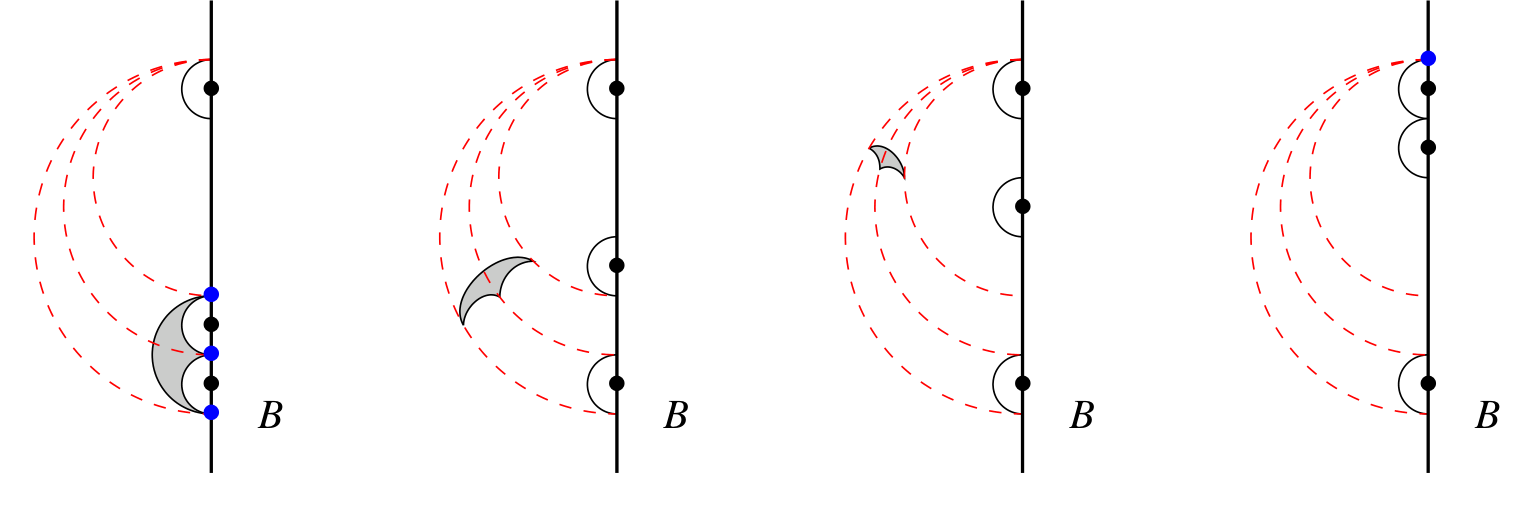
\includegraphics[width=0.92\linewidth]{figures/fig13.png}
  \caption{一个体开球与三个边界半开球的构型空间 $C_{\mathbb{H}^2}(1;3)$ 中的 $3$-链 $\mathcal{B}_3(\epsilon)$。蓝色顶点是 Figure 12 中四面体的顶点；灰色阴影区域是四面体的水平切片，其中最左侧的区域对应四面体的底面；红色虚线边是四面体的竖直边。（原文第 51 页，Figure 13）}
\end{figure}

\subsubsection{例：$B$ 型扭变的自由手征多重态}
% [背景补充: Hochschild 上同调 $HH^\bullet(A)$ 可理解为 $A$ 上恒等函子的导出自同态代数；具体计算使用上链复形 $\operatorname{Hom}(A^{\otimes n},A)$ 配 Hochschild 微分 $\delta$。其中 $HH^0(A)$ 是中心、$HH^1(A)$ 是外导子，这两条基本事实正是下文反复使用的入口。]
作为示例计算，考虑 $B$ 型扭变的自由手征多重态。在此情形下，边界条件的范畴由 $B$ 型 Neumann 边界条件生成。（用 Dirichlet 边界条件重新导出下面的结果也颇具启发性！\footnote{我们注意到，这两个基本边界条件各自都能生成 $B$ 型扭变自由手征多重态 TQFT 中边界条件的范畴，它们给出了 Koszul 对偶的一个简单实例。特别地，边界条件范畴中两个「横截（transverse）」生成对象 $B_1,B_2$，即满足 $\operatorname{Hom}(B_1,B_2)=\mathbb{C}$ 的生成元，支撑 Koszul 对偶的边界算子代数 [86, 87]。关于在镜像对称中有应用的更丰富的例子，参见 [88]，其中用到了导出 Fukaya–Seidel 范畴上的一个 Koszul 对偶版本；后者可看作由对应于左 thimble 或右 thimble 的边界条件所生成。}）局域算子代数就是多项式代数 $\mathbb{C}[\phi]$，因此我们关心 Hochschild 上同调 $HH^\bullet(\mathbb{C}[\phi])$。

如上所述，第零个 Hochschild 上同调群就是中心 $HH^0(A)\cong Z(A)$；由于 $\mathbb{C}[\phi]$ 是交换的，可得其 Hochschild 上同调群就是整个 $\mathbb{C}[\phi]$：
\begin{equation}
  \tag{3.50}
  HH^0(\mathbb{C}[\phi])\cong\mathbb{C}[\phi]\cong H^0(\mathbb{C}).
\end{equation}
% ==== 原文 PDF 第 52 页 ====
类似地，第一个 Hochschild 上同调群对应于代数的外导子 $HH^1(A)\cong\operatorname{OutDer}(A)$，即 $A$ 的导子（满足 $f(ab)=f(a)b\pm af(b)$ 的映射 $f:A\to A$）模去 $A$ 的内导子（由交换子给出的映射 $a\to[a,b]$，$b\in A$）。由于 $\mathbb{C}[\phi]$ 没有内导子，而 $\mathbb{C}[\phi]$ 的导子都形如 $\phi^k\partial_\phi$，可知 $HH^1(\mathbb{C}[\phi])$ 可等同为
% [存疑: 一般导子满足含符号的 Leibniz 法则 $f(ab)=f(a)b+(-1)^{|f||a|}af(b)$；原文此处写作 $\pm$，疑为把分次符号因子缩写掉了，语义上应读作含符号的 Leibniz 法则，照原文排印]
\begin{equation}
  \tag{3.51}
  HH^1(\mathbb{C}[\phi])\cong\mathbb{C}[\phi]\partial_\phi.
\end{equation}
其余 Hochschild 上同调群为零，故有
\begin{equation}
  \tag{3.52}
  HH^\bullet(\mathbb{C}[\phi])\cong\mathbb{C}[\phi]\oplus\mathbb{C}[\phi]\partial_\phi\cong H^{(0,\bullet)}(\mathbb{C},\wedge^\bullet T^{(1,0)}\mathbb{C}),
\end{equation}
% [Tutor Note: 对光滑仿射代数，Hochschild–Kostant–Rosenberg 定理给出 $HH^\bullet(A)\cong\wedge^\bullet\operatorname{Der}(A)$；对 $A=\mathbb{C}[\phi]$ 即得多向量场 $\mathbb{C}[\phi]\oplus\mathbb{C}[\phi]\partial_\phi$。右端的 $H^{(0,\bullet)}$ 把这一识别与复几何中全纯多向量场的 Dolbeault 型上同调对齐，从而与 2.3.2 节 $B$ 型扭变局域算子的描述衔接。]
它恰好与 $B$ 型扭变手征理论中局域算子的向量空间一致，参见 2.3.2 节。

Hochschild 上同调上的乘积结构由杯积 $\alpha\cup\beta$ 给出。具体而言，若 $\alpha$ 是 $p$-上链、$\beta$ 是 $(n-p)$-上链，则
\begin{equation}
  \tag{3.53}
  \alpha\cup\beta(O_1,\dots,O_n)=(-1)^{F(\alpha)(F(O_1)+\cdots+F(O_p))}\alpha(O_1,\dots,O_p)\beta(O_{p+1},\dots,O_n).
\end{equation}
% [Tutor Note: (3.53) 中的符号因子是 Koszul 符号：$\alpha$ 依次越过 $O_1,\dots,O_p$ 时每次交换贡献 $(-1)^{F(\alpha)F(O_i)}$，累乘即 $(-1)^{F(\alpha)(F(O_1)+\cdots+F(O_p))}$。若漏掉该因子，杯积的结合律会在奇次上链上差一个符号。]
例如 $\phi^k\cup\phi^l=\phi^{k+l}$，$\phi^k\cup\phi^l\partial_\phi=\phi^{k+l}\partial_\phi=\phi^k\partial_\phi\cup\phi^l$。更有意思的是，
\begin{equation}
  \tag{3.54}
  \partial_\phi\cup\partial_\phi(\phi^k,\phi^l)=kl\phi^{k+l-2}.
\end{equation}
% [Tutor Note: 按 (3.53) 取 $\alpha=\beta=\partial_\phi$，并用导子作用 $\partial_\phi(\phi^k)=k\phi^{k-1}$，即得 $kl\phi^{k+l-2}$；此处 $F(\partial_\phi)=1$、$F(\phi^k)=0$，故 Koszul 符号为 $+1$，与 (3.54) 的取值一致。]
注意这个 $2$-上链是 $\delta$-恰当的：
\begin{equation}
  \tag{3.55}
  \partial_\phi\cup\partial_\phi=-\delta(\partial_\phi^2),\qquad \partial_\phi^2(\phi^k)=k(k-1)\phi^{k-2},
\end{equation}
% [存疑: 按归一化 Hochschild 微分 $(\delta f)(a,b)=af(b)-f(ab)+f(a)b$ 直接计算，得 $\delta(\partial_\phi^2)(\phi^k,\phi^l)=-2kl\phi^{k+l-2}$，与 (3.55) 相差因子 $2$；可能源于原文采用的上链归一化或对称化约定，照原文排印]
因此 $\partial_\phi\cup\partial_\phi$ 在上同调层面为零，符合预期。这样我们不仅复原了局域算子的向量空间，也复原了其乘积结构。

这些考虑的一个近期应用可见于 [89, 90]：这些工作证明开–闭（type IIB 与 type I）拓扑弦具有唯一的量子化。作者用上同调论证证明了开–闭弦耦合中反常的抵消。在此背景下，刻画扭变 D 膜的一个（无穷）堆叠上开弦代数相容形变的 Hochschild 上同调（更确切地说，循环上同调；见脚注 23）重现了 BCOV 理论 [91]（扭变闭弦部分）给出的闭弦场空间。开弦代数可借助 D 膜世界体积理论的全纯 Chern–Simons 描述直接得到。可以通过与 BCOV 理论的耦合写出开弦理论的普适形变；参见我们在 3.2.6 节关于形变与下降的讨论。为边界条件范畴提供互补描述的 Koszul 对偶（见脚注 43）在这些背景中也起着作用 [11]：Koszul 对偶的代数具有相同的 Hochschild 上同调，因此可以用 Koszul 对偶过渡到开弦部分的另一种、可能更有用的描述。

\subsubsection{高维情形下的考虑}
存在于 $d=2$ 的许多结构可以更一般地推广到 $d\geq2$ 维的拓扑理论，参见 [73, Section 2]。局域算子的碰撞在 $Q$ 上同调类上诱导出结合且交换的乘积；
% ==== 原文 PDF 第 53 页 ====
3.1.3 节所述的次级乘积把这个交换代数提升为一个（$(1-d)$-移位的）Poisson 代数。在链层考虑这些运算，意味着该代数的各项性质只在由后代（descendant）编码的适当同伦意义下成立。这一概念被形式化为 $E_d$ 代数或 $d$-圆盘代数（$d$-disk algebra）[92]：对每一种插入点的选取都有一个乘积运算，此外还有联系同伦构型的数据；当 $d=1$ 时，$E_1$ 代数等价于 $A_\infty$ 代数。
% [背景补充: $E_d$（或 $d$-圆盘）代数由小圆盘操作子刻画：把 $n$ 个小圆盘嵌入一个大圆盘的不同构型给出 $n$ 元运算，各构型空间的分支之间由同伦数据粘合，这正是「运算只在同伦意义下成立」的形式化。]

若只关注次级乘积，即这个 $E_d$ 代数的 Lie 部分，则本质上\footnote{此外还有括号的分次斜对称性，但它不那么有意思。见 [73, Section 3.2.2]。}只需考虑一个关系：（移位后的）Jacobi 恒等式
\begin{equation}
  \tag{3.56}
  \{O_1,\{O_2,O_3\}\}=\{\{O_1,O_2\},O_3\}+(-1)^{(F(O_1)+1)(F(O_2)+1)}\{O_2,\{O_1,O_3\}\}.
\end{equation}
% [Tutor Note: 括号带有 $(1-d)$ 移位，故 Jacobi 恒等式中的符号不是未移位 Poisson 代数的 $(-1)^{F(O_1)F(O_2)}$，而是 $(-1)^{(F(O_1)+1)(F(O_2)+1)}$：把算子次数平移 $1$ 后可套用标准的 Koszul 符号（指数中 $\pm1$ 的差别为偶数，不改变符号），这正是「移位」在符号约定上的体现。]
上述链层考虑被编码在（移位后的）同伦 Lie 代数或 $L_\infty$ 代数\footnote{近期的工作 [48, 93] 在 $A$ 型扭变的有质量 Landau–Ginzburg 理论中得到次级乘积。包括次级乘积在内的代数结构被扩展为完整的 $L_\infty$ 结构。事实上，完整的体–边界系统具有更大的同伦代数结构，其中包含与边界局域算子代数相联系的 $A_\infty$ 代数，称为 $LA_\infty$ 代数，并且人们相信它还会进一步强化为完整的 $E_2$ 代数结构。我们就这一点与 G. Moore 和 A. Khan 的通信表示感谢。（这些理论中还有描述二维中一维拓扑线融合的 $A_\infty$ 结构，它与 2d TQFT 的 $(\infty,2)$-范畴结构相联系。）体–边界系统中的同伦代数也在开–闭弦场论的背景下被考虑过，例如 [94]。}的概念之中。例如在 $d=2$ 时，可定义如下三元运算 $\ell_3$：给定 $\mathbb{R}^2$ 上的三个点（开球），考虑 Figure 14 中所示的区域。由此在构型空间 $C_{\mathbb{R}^2}(3)$ 中得到的 $3$-链 $\mathcal{L}_3$ 是一个挖去两个实心环面的实心环面（solid torus）。给定 $Q$-闭的局域算子 $O_1,O_2,O_3$，考虑由此得到的乘积
\begin{equation}
  \tag{3.57}
  \ell_3(O_1,O_2,O_3)=\int_{\mathcal{L}_3}(O_1O_2O_3)^{(3)}=\int_{\mathcal{L}_3}O_1^{(2)}O_2^{(1)}O_3.
\end{equation}
% [Tutor Note: (3.57) 的第二个等号由下降方程逐项作用得到：$(O_1O_2O_3)^{(3)}=O_1^{(2)}O_2^{(1)}O_3$；其中 $O_1^{(2)}$ 沿二维区域 $D$ 积分、$O_2^{(1)}$ 沿环绕点 $w$ 的围道积分，而 $O_3$ 置于该围道内的点 $w$ 处，三者共同张成 $C_{\mathbb{R}^2}(3)$ 中的 $3$-链 $\mathcal{L}_3$。]
直接的计算表明
\begin{equation}
  \tag{3.58}
  \begin{aligned}
  Q\ell_3(O_1,O_2,O_3)={}&\{O_1,\{O_2,O_3\}\}-\{\{O_1,O_2\},O_3\}\\
  &-(-1)^{(F(O_1)+1)(F(O_2)+1)}\{O_2,\{O_1,O_3\}\},
  \end{aligned}
\end{equation}
% [Tutor Note: (3.58) 的右端正是把 (3.56) 的右端减去其左端所得的 Jacobi 残差，故 $\ell_3$ 给出该恒等式的同伦：它把链层的 Jacobi 残差写成 $Q$-恰当项，从而在 $Q$-上同调层面该残差为零。这也正是 $L_\infty$ 结构中三阶运算 $\ell_3$ 的地位：它本身不是括号，而是括号结合律（此处为 Jacobi 恒等式）的同伦修正。]
从而 $\ell_3(O_1,O_2,O_3)$ 是把（移位后的）Jacobi 恒等式平凡化的一个同伦。类似地，更高的 $n$ 元 $L_\infty$ 乘积可以通过在 $\mathbb{R}^2$ 上 $n$ 个点的构型空间中沿闭链积分来实现。

同样可以从对理论边界条件的充分了解中复原体局域算子代数。事实上，这是 Baez–Dolan 配边假设（cobordism hypothesis）[95] 的一个极简实例；该假设本质上说，一个 $d$ 维 TQFT 完全由其 $(d-1)$-范畴的边界条件确定（在同伦意义下）；另见 [92]。

有一种情形只需要少得多的信息就能走得很远：3 维 TQFT 容许一个（足够大的）全纯边界条件，从而提供顶点算子代数（VOA）。原型例子是 Chern–Simons 理论与边界 Wess–Zumino–Witten（WZW）流代数之间的经典联系 [96]；这一情形也适用于 3.1.2 节所述的 $A$ 型与 $B$ 型扭变的 $N=4$ 理论 [97]。
% [存疑: 原文此处 $N$ 为普通斜体，与全文其他处 $\mathcal{N}$ 的写法不一致；已照原样排印]
在此情形下，体 TQFT 的局域算子代数可实现为边界 VOA（在球面上）的共形块空间，在导出（derived）情形下也称为手征同调（chiral homology）[98]；
% ==== 原文 PDF 第 54 页 ====
WZW 流代数只有一个共形块，这对应于体中局域算子的缺失；而对于扭变 3 维 $N=4$ 理论 [99] 中出现的 VOA，共形块通常有无穷多个，以容纳 Higgs 分支与 Coulomb 分支上（通常为无穷维的）全纯函数代数。

% [说明: 原文 Figure 14 位于第 54 页页首；此处按浮动体 [t] 放置以复现原版位]
\begin{figure}[tbp]
  \centering
  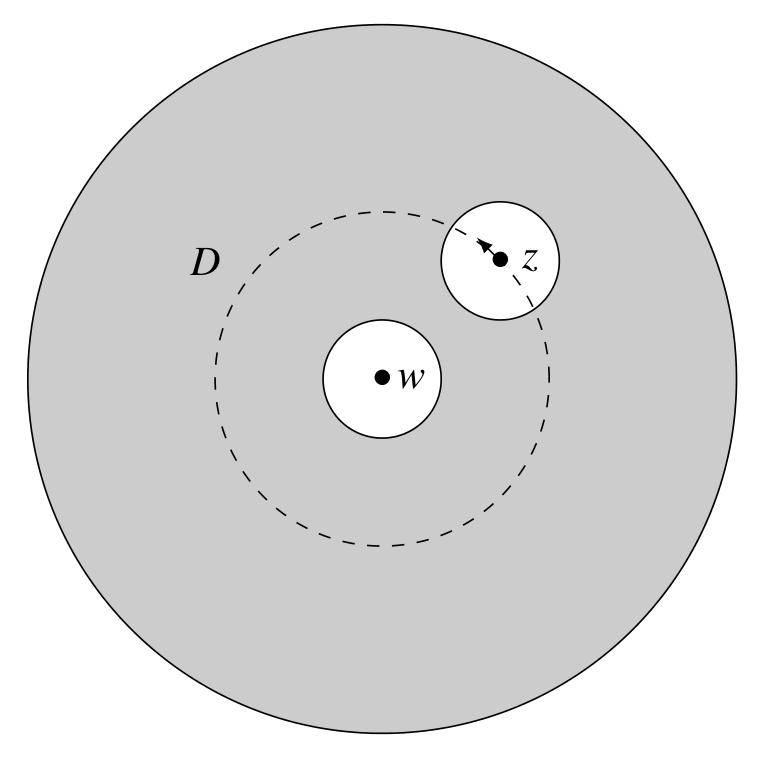
\includegraphics[width=0.92\linewidth]{figures/fig14.png}
  \caption{用于构造三元乘积 $\ell_3$ 的、构型空间 $C_{\mathbb{R}^2}(3)$ 中 $3$-闭链 $\mathcal{L}_3$ 的一个切片。局域算子 $O_3$ 置于点 $w$，取值 $1$-形式的局域算子 $O_2^{(1)}$ 置于点 $z$，取值 $2$-形式的局域算子 $O_1^{(2)}$ 置于点 $u$。变量 $u$ 在二维区域 $D$ 上积分，$z$ 沿环绕 $w$ 的虚线围道积分。（原文第 54 页，Figure 14）}
\end{figure}

\subsubsection{关于高阶代数与形变的简要说明}
关于高阶代数可谈的内容很多，我们只触及了表面。其中一条重要的思路——遗憾的是我们只能简短提及——是数学中形式形变（或模）问题与同伦 Lie 代数、同伦结合代数之间的深刻联系。

这一联系如下产生。考虑 DG-Lie 代数 $(A,d_A)$ 的 Maurer–Cartan（MC）方程的解；所谓 DG-Lie 代数，即分次 Lie 代数 $(A=\bigoplus A^j,[-,-])$ 带一个微分 $d_A:A^j\to A^{j+1}$，且满足幂零性 $d_A^2=0$：
\begin{equation}
  \tag{3.59}
  d_Ax+\frac{1}{2}[x,x]=0,\qquad x\in A.
\end{equation}
% [Tutor Note: 展开 $(d_A+[x,\cdot])^2=0$，利用 $d_A$ 是导子、$d_A^2=0$ 与分次 Jacobi 恒等式，得 $[d_Ax+\frac{1}{2}[x,x],\cdot]=0$；系数 $1/2$ 正是分次反对称性导致的重复计数。于是 MC 方程即「一阶形变不破坏幂零性」的条件，其解模去规范等价后就是 DG-Lie 代数的形变空间。]
该方程可看作一个要求：在存在一阶形变 $d_A+[x,\cdot]$ 时，微分仍保持幂零。该方程的解空间等价于 DG-Lie 代数的（微扰）形变空间。对 DG-结合代数也有类似的 MC 方程，其中二次项由结合乘积给出。更一般地，可以为同伦代数写出 MC 方程，其中二次项被替换为对所有更高 $n$ 元运算（$n\geq2$）的求和。

Maurer–Cartan 方程在物理中相当普遍地出现。乍看之下，它们在 Chern–Simons 型或 BF 型理论中就是运动方程，因而并不陌生。例如，弦场论研究者会认出 MC 方程正是（开–）闭弦场论的运动方程。在这一背景下，运动方程的解描述闭弦背景，其解释是围绕给定几何背景（即真空解）的相容形变。
